% Software Impacts -- Original Software Publication (draft)
%
% Elsevier's `elsarticle` class is used when it is installed (it is on Overleaf and in TeX Live
% "full"). Otherwise a minimal stand-in lets you compile a *preview* of this draft; the layout
% of the stand-in is NOT the journal layout.
%
% Build:   latexmk -pdf main.tex        (needs references.bib and, optionally, results.tex)
% Figures: python figures/make_figures.py
% Table:   python ../benchmarks/make_report.py ../benchmarks/results <part folders>
%          (writes ../benchmarks/results/results.tex, see ../benchmarks/README.md)
%
% Every number in this draft was measured with the repository (benchmarks/results/REPORT.md,
% docs/explainability.md, docs/limitations.md); none is a target or an estimate.
\IfFileExists{elsarticle.cls}{%
  \documentclass[review,12pt]{elsarticle}%
}{%
  \documentclass[11pt,a4paper]{article}%
  % Stand-in for Elsevier's `elsarticle` front-matter commands, used only to preview the draft when
% elsarticle.cls is not installed. The journal layout is NOT reproduced.
\usepackage[margin=2.3cm]{geometry}
\usepackage{natbib}
\makeatletter
\renewcommand{\title}[1]{\begin{center}{\Large\bfseries #1\par}\end{center}}
\renewcommand{\author}[2][]{\begin{center}#2\end{center}\vspace{-1.2em}}
\newcommand{\address}[2][]{\begin{center}\small\itshape #2\end{center}\vspace{-1.2em}}
\newenvironment{frontmatter}{}{}
\newcommand{\ead}[1]{}
\newcommand{\fntext}[2][]{}
\newenvironment{keyword}{\par\noindent\textbf{Keywords:} }{\par}
\newcommand{\sep}{; }
\makeatother
%
}

\usepackage{graphicx}
\usepackage{booktabs}
\usepackage{array}
\usepackage{listings}
\usepackage[hidelinks]{hyperref}
\usepackage{xcolor}
\lstset{basicstyle=\ttfamily\footnotesize, breaklines=true, columns=fullflexible,
        keepspaces=true, frame=single, rulecolor=\color{black!30}}
\newcommand{\todo}[1]{\textcolor{red}{[TODO: #1]}}
\newcommand{\amlgm}{\textsc{AML-GraphMiner}}

\begin{document}

\begin{frontmatter}

\title{\amlgm: an open-source toolkit for explainable money-laundering detection on transaction graphs}

% --- authors: fill in before submission -------------------------------------------------------
\author[fst]{\todo{Student name}}
\author[urk]{Mohamedou El Ghotob Cheikh Tourad}
\address[fst]{Faculty of Sciences and Techniques, University of Nouakchott, Mauritania}
\address[urk]{Al-Khawarizmi Research Unit, University of Nouakchott, Mauritania}

\begin{abstract}
Money laundering moves an estimated 2--5\,\% of world GDP every year, yet anti-money-laundering
(AML) systems still rely on proprietary rule engines that bury investigators in false alerts, while
the graph neural networks (GNNs) proposed in research are hard to reproduce and seldom explained.
\amlgm{} is an open-source Python toolkit that unifies the two worlds on transaction graphs. It
ingests the IBM AML and Elliptic benchmarks or any CSV/JSON/Parquet table into one validated schema,
builds leak-free temporal features, detects six classical laundering motifs and risk communities
with auditable evidence, trains tabular baselines, GCN, GraphSAGE, GAT and a label-free graph
auto-encoder under one temporal protocol, stacks any model with the motifs, and explains every alert
through pattern evidence, occlusion, GNNExplainer, PGExplainer, Captum and attention, reporting how
much the neighbourhood really changes the score. A web investigation interface, a command line, a
REST API, MLflow, Hugging Face Hub and Neo4j exports, notebooks and benchmark scripts make studies
reproducible. On IBM AML HI-Small (0.18\,\% laundering), GraphSAGE reaches a test PR-AUC of 0.531,
the untrained motif scanner 0.340 and a random forest stacked with the motifs 0.562. The toolkit targets researchers, teachers and institutions, such as regional banks, that
cannot afford commercial AML suites.
\end{abstract}

\begin{keyword}
anti-money laundering \sep graph neural networks \sep open-source \sep financial crime \sep explainable AI
\end{keyword}

\end{frontmatter}

\section*{Code metadata}
\begin{table}[h]
\centering
\small
\begin{tabular}{@{}l p{4.2cm} p{7.2cm}@{}}
\toprule
\textbf{Nr.} & \textbf{Code metadata description} & \textbf{Value} \\
\midrule
C1 & Current code version & v0.1.0 \\
C2 & Permanent link to code/repository used for this code version & \todo{public GitHub URL and Zenodo DOI of the archived release (the repository is private until submission)} \\
C3 & Permanent link to Reproducible Capsule & \todo{optional (e.g.\ Code Ocean)} \\
C4 & Legal Code License & MIT \\
C5 & Code versioning system used & git \\
C6 & Software code languages, tools, and services used & Python 3.11+, JavaScript (web interface); PyTorch, PyTorch Geometric, PyTorch Lightning, Captum, scikit-learn, XGBoost, NetworkX, pandas, Pydantic, Click, FastAPI, MLflow, Neo4j driver; pytest, Hypothesis, GitHub Actions, Sphinx, Docker \\
C7 & Compilation requirements, operating environments \& dependencies & Linux (reference), macOS, Windows; the core installs without PyTorch; GNN training needs \texttt{aml-graphminer[gnn]} and the \texttt{pyg-lib} wheel; GPU optional \\
C8 & Link to developer documentation/manual & \todo{Read the Docs URL} \\
C9 & Support email for questions & \todo{maintainer e-mail} \\
\bottomrule
\end{tabular}
\end{table}

\section{Motivation and significance}

Money laundering hides the proceeds of crime in the volume of legitimate payments. The United
Nations Office on Drugs and Crime estimated the funds laundered in 2009 at about 1.6 trillion US
dollars, 2.7\,\% of world GDP, in line with the 2--5\,\% range of earlier International Monetary
Fund estimates \cite{unodc2011illicit}. Financial institutions must detect and report suspicious
activity under the FATF Recommendations \cite{fatf2012recommendations}, transposed in West Africa by
Directive n\textsuperscript{o}\,02/2015/CM/UEMOA and the uniform law applied under the BCEAO
\cite{uemoa2015directive}. Detection is a needle-in-a-haystack problem
--- 0.18\,\% of the test transactions of the IBM AML HI-Small benchmark are laundering
\cite{altman2023realistic} --- and an alert is only useful if an analyst can see \emph{why} it was
raised. Rule engines saturate investigators with false positives, while deep models that cannot
justify a decision are hard to accept for supervisors \cite{fatf2021newtech}.

Graph methods suit the problem because laundering schemes are relational: funds are split, layered
through intermediaries and gathered again. GNNs such as GCN \cite{kipf2017semi}, GraphSAGE
\cite{hamilton2017inductive} and GAT \cite{velickovic2018graph} have been applied to Bitcoin
\cite{weber2019anti} and to synthetic bank data produced by simulators such as AMLSim
\cite{weber2018scalable}, the IBM AMLworld generator \cite{altman2023realistic} or, recently, Tide
\cite{vandenbeukel2026tide}, with dedicated architectures \cite{egressy2024provably,cardoso2022laundrograph}.
Yet studies are rarely comparable: each re-implements its own pipeline, splits are random rather
than temporal, features are fitted on all data, and explanations are an afterthought. No
open-source toolkit puts deterministic typology detectors, learned models and explanations behind
one protocol. \amlgm{} fills that gap: it is a tested library, not a notebook, and every number
quoted below can be regenerated with one command.

\section{Software description}

\paragraph{Architecture} The code is organised in six layers (Fig.~\ref{fig:arch}): ingestion
(adapters for IBM AML, Elliptic and generic tables, Pydantic validation, parser of the IBM laundering
annotations), features (causal trailing windows of 1\,h, 24\,h and 7\,d, PageRank, degrees,
velocity, fitted on the training period only), graph (NetworkX, PyTorch Geometric
\cite{fey2019fast} and heterogeneous representations, Neo4j export), detectors, explainers and
interfaces. Each layer depends only on those below; heavy dependencies (PyTorch, FastAPI, Captum)
are optional extras imported lazily, so the core runs on a laptop without a GPU. Tabular models use
scikit-learn \cite{pedregosa2011scikit} and XGBoost; graph algorithms use NetworkX
\cite{hagberg2008exploring}.

\begin{figure}[t]
\centering
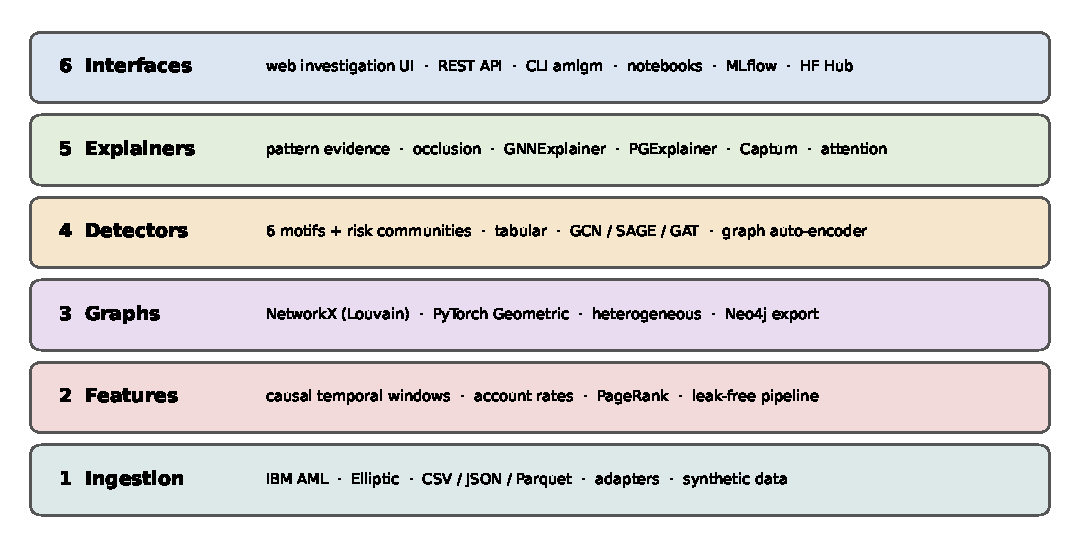
\includegraphics[width=0.92\linewidth]{figures/architecture.pdf}
\caption{The six layers of \amlgm. Every interface (web interface, CLI, REST API, notebooks) is a
thin wrapper around the same Python SDK.}
\label{fig:arch}
\end{figure}

\paragraph{Detectors} Six motif detectors --- fan-in, fan-out, smurfing, time-respecting cycles,
scatter-gather, gather-scatter --- and a risk-community detector (relay accounts, Louvain
\cite{blondel2008fast}) need no training; each alert carries its accounts, transactions and
numbers. Amounts are converted to a reference currency with exchange rates inferred from the
cross-currency transactions themselves, and a time slice is scanned with the preceding days as
unlabelled context, so a motif that changes currency or straddles the start of the slice is still
seen whole. Learned detectors are logistic regression, random forest, gradient boosting, XGBoost,
GCN, GraphSAGE and GAT edge classifiers with neighbour sampling and a graph auto-encoder trained
without labels \cite{kipf2016variational,ding2019deep}. A hybrid detector stacks any of them with
the motif scanner (a three-coefficient logistic regression fitted on validation). All share one
interface (\texttt{fit}, \texttt{score}, \texttt{predict}, \texttt{save}, \texttt{load}) and one
on-disk format --- a \texttt{config.json} with the feature statistics, threshold and test metrics
next to the weights --- which \texttt{amlgm export-hub} turns into a Hugging Face Hub repository with
a generated model card.

\paragraph{Configuration} Detectors are configured in YAML, validated when the file is loaded
(unknown keys and malformed durations fail early):

\begin{lstlisting}
patterns:
  fan_in:  {min_counterparties: 3, window: 120h, min_burst_ratio: 0}
  cycle:   {max_length: 12, max_span: 4d, min_hop_ratio: 0.5, max_hop_ratio: 1.5}
  currency: {convert: true, reference: US Dollar}
  lookback: 4d                  # unlabelled context before a scored slice
  transaction_types: [ACH]
\end{lstlisting}

\paragraph{Protocol and explanations} Transactions are split by time (60/20/20); statistics and
thresholds are fitted on training and validation only, enforced by unit tests that alter future
data. Alerts are explained by pattern evidence, occlusion of neighbouring transactions and
accounts, GNNExplainer \cite{ying2019gnnexplainer}, PGExplainer \cite{luo2020parameterized},
Integrated Gradients \cite{sundararajan2017axiomatic} through Captum \cite{kokhlikyan2020captum}
and GAT attention. Every method returns the same \texttt{Explanation} object (signed importance of
neighbouring transactions, accounts and features, motifs involved), serialisable to JSON, Markdown
and NetworkX; GNN explanations also report the measured score with and without the neighbourhood.
The pipeline from loading to explanation fits in a few lines:

\begin{lstlisting}[language=Python]
import aml_graphminer as aml
from aml_graphminer.detectors.bundle import MotifDetector, TabularDetector
from aml_graphminer.explainers import explain_alerts

df = aml.load_dataset("data/HI-Small_Trans.csv")   # + laundering annotations
motifs = MotifDetector.fit(df)                     # calibrated on validation
model = TabularDetector.fit(df, "hgb")             # temporal split, leak-free
print(model.metrics)                               # test metrics
case = explain_alerts(model, df, top=20, out_dir="case/")
\end{lstlisting}

\section{Illustrative examples}

The three examples are the executed notebooks of the repository.

\paragraph{(1) Quick start} \texttt{01\_quickstart} runs the whole toolkit on the bundled synthetic
generator (no download): motif and community alerts, a gradient-boosting model, its explanation and
the label-free auto-encoder. The same session is \texttt{amlgm scan}, \texttt{amlgm train} and
\texttt{amlgm explain} on the command line, and \texttt{amlgm serve --demo} opens it in a browser.

\paragraph{(2) Benchmark} \texttt{02\_ibm\_aml\_benchmark} and \texttt{benchmarks/run\_ibm.py}
compare every detector on IBM AML HI-Small and LI-Small (5.08 and 6.92 million transactions) and
on Elliptic (Table~\ref{tab:results}). On HI-Small GraphSAGE reaches a test PR-AUC of
$0.531\pm0.022$ over three seeds, ahead of the random forest ($0.499\pm0.017$); on the harder
LI-Small file (prevalence 0.067\,\%) the random forest leads ($0.191\pm0.007$). The motif scanner
alone, without any training and tuned on validation only, reaches 0.340 on HI-Small and 0.147 on
LI-Small --- below the best learned models, above logistic regression, and on LI-Small above
HistGradientBoosting, GCN and GAT --- with exact, auditable alerts. Currency conversion and the
unlabelled history context are what make this possible: without them the same scanner reached
0.005 and 0.001, its cycle detector recovering none of the annotated cycles (0.81 of them on
HI-Small now). Stacking a saved model with the motifs raises the HI-Small test PR-AUC from 0.519
to 0.562 for a random forest and from 0.504 to 0.527 for GraphSAGE (one seed), but brings nothing
on LI-Small (0.191 to 0.186 for the random forest). On Elliptic the
tree models (PR-AUC about 0.79) clearly beat the GNNs (GraphSAGE $0.497\pm0.056$), which shows
why the toolkit always reports both.

\IfFileExists{../benchmarks/results/results.tex}{%
\begin{table}[t]
\centering\scriptsize
% Generated by benchmarks/make_report.py — do not edit by hand.
\begin{tabular}{llrrrrr}
\toprule
Dataset & Model & PR-AUC & F1 & Precision & Recall & Recall@k \\
\midrule
HI-Small & sage & 0.531 $\pm$ 0.022 & 0.510 $\pm$ 0.035 & 0.834 $\pm$ 0.012 & 0.368 $\pm$ 0.035 & 0.513 $\pm$ 0.021 \\
 & rf & 0.499 $\pm$ 0.017 & 0.563 $\pm$ 0.006 & 0.839 $\pm$ 0.015 & 0.424 $\pm$ 0.010 & 0.492 $\pm$ 0.018 \\
 & hgb & 0.476 $\pm$ 0.011 & 0.507 $\pm$ 0.005 & 0.740 $\pm$ 0.019 & 0.386 $\pm$ 0.001 & 0.470 $\pm$ 0.013 \\
 & xgb & 0.474 $\pm$ 0.005 & 0.441 $\pm$ 0.019 & 0.742 $\pm$ 0.054 & 0.315 $\pm$ 0.029 & 0.459 $\pm$ 0.003 \\
 & gat & 0.447 $\pm$ 0.007 & 0.387 $\pm$ 0.028 & 0.872 $\pm$ 0.035 & 0.250 $\pm$ 0.025 & 0.452 $\pm$ 0.007 \\
 & gcn & 0.374 $\pm$ 0.031 & 0.363 $\pm$ 0.029 & 0.785 $\pm$ 0.036 & 0.236 $\pm$ 0.022 & 0.389 $\pm$ 0.030 \\
 & patterns & 0.340 & 0.392 & 0.405 & 0.380 & 0.386 \\
 & logreg & 0.294 $\pm$ 0.000 & 0.352 $\pm$ 0.000 & 0.334 $\pm$ 0.000 & 0.373 $\pm$ 0.000 & 0.349 $\pm$ 0.000 \\
 & gae & 0.003 $\pm$ 0.001 & 0.006 $\pm$ 0.001 & 0.003 $\pm$ 0.001 & 0.480 $\pm$ 0.047 & 0.002 $\pm$ 0.001 \\
\midrule
LI-Small & rf & 0.191 $\pm$ 0.007 & 0.260 $\pm$ 0.005 & 0.561 $\pm$ 0.084 & 0.170 $\pm$ 0.012 & 0.231 $\pm$ 0.007 \\
 & sage & 0.176 $\pm$ 0.018 & 0.219 $\pm$ 0.023 & 0.646 $\pm$ 0.156 & 0.135 $\pm$ 0.026 & 0.200 $\pm$ 0.018 \\
 & patterns & 0.147 & 0.172 & 0.154 & 0.195 & 0.184 \\
 & gat & 0.110 $\pm$ 0.026 & 0.135 $\pm$ 0.026 & 0.468 $\pm$ 0.168 & 0.080 $\pm$ 0.013 & 0.149 $\pm$ 0.021 \\
 & hgb & 0.106 $\pm$ 0.016 & 0.157 $\pm$ 0.006 & 0.172 $\pm$ 0.060 & 0.160 $\pm$ 0.040 & 0.154 $\pm$ 0.007 \\
 & xgb & 0.078 $\pm$ 0.007 & 0.150 $\pm$ 0.015 & 0.153 $\pm$ 0.007 & 0.149 $\pm$ 0.023 & 0.150 $\pm$ 0.008 \\
 & gcn & 0.074 $\pm$ 0.024 & 0.108 $\pm$ 0.037 & 0.234 $\pm$ 0.100 & 0.078 $\pm$ 0.033 & 0.124 $\pm$ 0.016 \\
 & logreg & 0.032 $\pm$ 0.000 & 0.082 $\pm$ 0.000 & 0.063 $\pm$ 0.000 & 0.117 $\pm$ 0.000 & 0.076 $\pm$ 0.000 \\
 & gae & 0.001 $\pm$ 0.000 & 0.003 $\pm$ 0.001 & 0.001 $\pm$ 0.000 & 0.471 $\pm$ 0.079 & 0.001 $\pm$ 0.001 \\
\midrule
elliptic & hgb & 0.790 $\pm$ 0.004 & 0.756 $\pm$ 0.037 & 0.798 $\pm$ 0.083 & 0.721 $\pm$ 0.003 & 0.729 $\pm$ 0.005 \\
 & xgb & 0.788 $\pm$ 0.002 & 0.762 $\pm$ 0.021 & 0.792 $\pm$ 0.050 & 0.735 $\pm$ 0.004 & 0.739 $\pm$ 0.001 \\
 & rf & 0.786 $\pm$ 0.001 & 0.791 $\pm$ 0.007 & 0.877 $\pm$ 0.019 & 0.721 $\pm$ 0.002 & 0.733 $\pm$ 0.002 \\
 & sage & 0.497 $\pm$ 0.056 & 0.566 $\pm$ 0.021 & 0.570 $\pm$ 0.017 & 0.563 $\pm$ 0.026 & 0.566 $\pm$ 0.023 \\
 & gat & 0.351 $\pm$ 0.042 & 0.398 $\pm$ 0.023 & 0.336 $\pm$ 0.049 & 0.496 $\pm$ 0.032 & 0.407 $\pm$ 0.010 \\
 & gcn & 0.300 $\pm$ 0.055 & 0.382 $\pm$ 0.040 & 0.387 $\pm$ 0.059 & 0.378 $\pm$ 0.024 & 0.381 $\pm$ 0.058 \\
 & logreg & 0.209 $\pm$ 0.000 & 0.324 $\pm$ 0.000 & 0.202 $\pm$ 0.000 & 0.812 $\pm$ 0.000 & 0.241 $\pm$ 0.000 \\
\bottomrule
\end{tabular}

\caption{Test-split results generated by \texttt{benchmarks/make\_report.py}: IBM AML HI-Small and
LI-Small (temporal 60/20/20 split; mean $\pm$ standard deviation over three seeds; motif thresholds
tuned on the validation split only; tabular models and motifs on a laptop CPU, GNNs on a Kaggle T4
GPU) and Elliptic (node classification, time steps 1--29 / 30--34 / 35--49). Test prevalence:
0.177\,\% (HI-Small), 0.067\,\% (LI-Small), 6.5\,\% (Elliptic).}
\label{tab:results}
\end{table}
}{%
\par\medskip\noindent\fbox{\parbox{0.95\linewidth}{\small\todo{Benchmark table: run
\texttt{benchmarks/make\_report.py}; it writes \texttt{benchmarks/results/results.tex}, which this
paper includes automatically.}}}\par\medskip
}

\paragraph{(3) Explaining an alert} \texttt{03\_explainability} investigates alerts with every
method. Figure~\ref{fig:expl} shows the exact evidence of a transaction flagged by the cycle
detector. For the GraphSAGE model trained on HI-Small, the toolkit's neighbourhood check shows
that the eight highest-scored test transactions keep a score of 0.960--1.000 when their
neighbouring transactions are removed (0.988--1.000 with them), and removing the five neighbours
ranked first by GNNExplainer leaves the score unchanged: the decision rests on the transaction and
the profiles of its accounts. PGExplainer accordingly returns empty masks, and feature attributions
(Captum) are the informative view --- a finding that would go unnoticed if the edge masks were
shown without this check.

\begin{figure}[t]
\centering
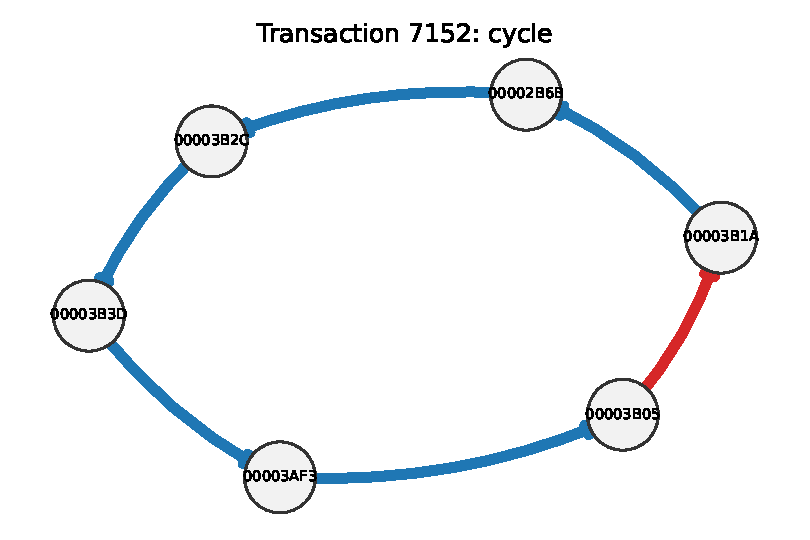
\includegraphics[width=0.62\linewidth]{figures/example_explanation.pdf}
\caption{Pattern explanation of one transaction (red) on \emph{synthetic} data: it belongs to a
laundering cycle through three accounts in which the amount is almost conserved.}
\label{fig:expl}
\end{figure}

\section{Impact}

\emph{Academic.} Each AML/GNN study currently rebuilds its pipeline; \amlgm{} gives a reusable,
tested one (more than 450 tests, 98\,\% line coverage, typed, continuous integration) with the
temporal protocol, seeds, configuration and library versions stored next to every result, so a
comparison can be rerun or extended with one command. New motifs, input formats and explainers are
added through small registries without touching the rest of the pipeline. \emph{Teaching.} The
synthetic generator, the executed notebooks and the web interface let students explore laundering
typologies, detectors, explanations and evaluation pitfalls without access to bank data.
\emph{Industrial.} Fintechs and regional banks that cannot license commercial suites get detectors
that run on a laptop, can be served through a REST API and investigated in a browser.
\emph{Regulatory.} Motif alerts carry their own evidence and every model alert can be explained and
exported to a case file, which addresses the explainability expected by supervisors
\cite{fatf2021newtech}. \emph{Geographic.} The software originates at the University of Nouakchott;
being free and light, it is accessible to institutions of the UEMOA/ECOWAS region and other
developing economies. \todo{Add a sourced figure for the size of the AML software market and list
publications and projects that use the software once they exist.}

\section{Conclusions}

\amlgm{} unifies deterministic typology detection, learned graph models, their combination and
their explanation behind one leak-free temporal protocol and four interfaces. Measured on the public
benchmarks, it reproduces the strength of GNNs on IBM AML HI-Small, shows where tree models remain
better (LI-Small, Elliptic), shows that typology rules become useful once amounts are compared
across currencies and motifs are seen whole (alone, and stacked with a model on HI-Small), and
exposes the limits of edge-mask explanations instead of hiding them. The IBM data are synthetic, so scores measure how well a
method recovers the generator's motifs, not real-world performance; motif settings must be retuned
on institutional data (the restriction to ACH transfers chosen on IBM validation data is a property
of that simulator); the REST API has no authentication. Future work includes heterogeneous and
temporal GNNs, directed-multigraph GNNs \cite{egressy2024provably}, privacy-preserving training
across banks (federated learning) and validation on real data with a partner institution.

\section*{Acknowledgements}
\todo{Funding, supervision, data providers (IBM, Elliptic).}

\section*{Declaration of competing interest}
\todo{Confirm with the authors; the template of the journal requires this statement.}

\section*{Declaration of generative AI and AI-assisted technologies in the writing process}
\todo{Check the journal's current policy and state any use of AI assistance in code or text accurately.}

\IfFileExists{elsarticle-num.bst}{\bibliographystyle{elsarticle-num}}{\bibliographystyle{plainnat}}
\bibliography{references}

\end{document}
